

The escalation of complex machine learning models across various domains has prompted the development of visual analytics tools designed to make these models more interpretable and trustworthy. While the theoretical foundations of eXplainable Artificial Intelligence have been extensively studied, the practical implementation of these concepts through interactive visual systems represents a critical need to connect the algorithmic explanations to human understanding \cite{8807299,analytics4010007}.

As highlighted by Spinner et al.\cite{8807299}, there exists a significant gap between theoretical XAI frameworks and their use in practical systems that support real-world model development and deployment workflows. This gap becomes particularly pronounced when considering the diverse user groups that interact with machine learning models, from domain experts with limited technical background to experienced data scientists in need of algorithmic insights \cite{Z_ller_2023}.

The landscape of XAI visual analytics tools has evolved to address different aspects of the explainability challenge, ranging from comprehensive frameworks that integrate multiple explanation methods \cite{8807299} to specialized tools that focus on specific explanation paradigms such as local explanations \cite{9861728,cappuccio2024fipervisualbasedexplanationcombining} or surrogate model visualization \cite{Chatzimparmpas2023DeforestVisBA}. However, most existing approaches tend to address either global model understanding or local instance explanations, and in the latter case, they rarely provide integrated views that make the relationship between the generated neighborhood and the resulting explanation obvious.

In the context of this thesis, which focuses on developing an interactive explanation system for 
% the $\text{LORE}_{sa}$ algorithm
explainability methods which involve both a synthetically generated neighborhood and a surrogate model, 
understanding the current state of visual eXplainable Artificial Intelligence tools is crucial. The integration of dimensionality reduction techniques (such as UMAP projections) with decision tree visualization presents specific design challenges that few existing tools have addressed.

This section examines the current state of the art of XAI visual analytics tools, organizing them into several categories based on their primary focus and methodological approach. We analyze comprehensive frameworks that attempt to unify multiple XAI methods \cite{8807299,Z_ller_2023}, specialized tools for local explanation analysis \cite{9861728,cappuccio2024fipervisualbasedexplanationcombining}, surrogate model visualization approaches \cite{Chatzimparmpas2023DeforestVisBA}, and industrial deployment considerations \cite{analytics4010007}.

Through this analysis, we identify key design patterns, interaction paradigms, and visualization techniques that inform the development of effective interfaces.
% for $\text{LORE}_{sa}$ explanations. 
Particular attention is paid to tools that employ scatter plot visualizations for neighborhood representation and surrogate model interfaces for rule exploration, as these components are central to the proposed system. Furthermore, we examine how existing tools handle the coordination between different explanation views and support user interaction workflows that allow both exploratory analysis and targeted explanation refinement.

\subsubsection{Comprehensive XAI Visual Analytics Frameworks}

Comprehensive XAI visual analytics frameworks represent an ambitious approach to addressing the XAI field. Unlike specialized tools that focus on particular explanation methods or user scenarios, comprehensive frameworks attempt to integrate multiple XAI techniques within unified platforms that support diverse workflows and user needs. Two notable examples are \textbf{explAIner} and \textbf{XAutoML}, each addressing different aspects of the machine learning lifecycle while providing comprehensive approaches to model understanding and confirmation.

\paragraph{explAIner: Interactive Deep Learning Model Analysis}

This 
% \textbf{explAIner} 
framework \cite{8807299} presents a complete approach to interactive and eXplainable Artificial Intelligence, specifically designed for deep learning models and integrated in the TensorBoard ecosystem. The framework is built around an iterative XAI pipeline that structures the explanation process into three core phases: \textit{understanding}, \textit{diagnosis}, and \textit{refinement}. 

The central concept in this framework are the \textit{explainers}, which serve as a modular building block that take one or more model states as input, applies an XAI method, and outputs either explanations (visualizations, verbalizations, surrogate models) or transition functions for model refinement. The framework distinguishes between single-model explainers that analyze individual model states and multi-model explainers that perform comparative analysis across different model configurations. This modular design enables the integration of diverse explanation methods including LIME \cite{ribeiro2016should}, LRP \cite{Bach2015OnPE}, SHAP \cite{lundberg2017unified}, gradient-based methods, and custom implementations.

\begin{figure}
    \centering
    \begin{subfigure}[c]{0.6\textwidth}
        \centering
        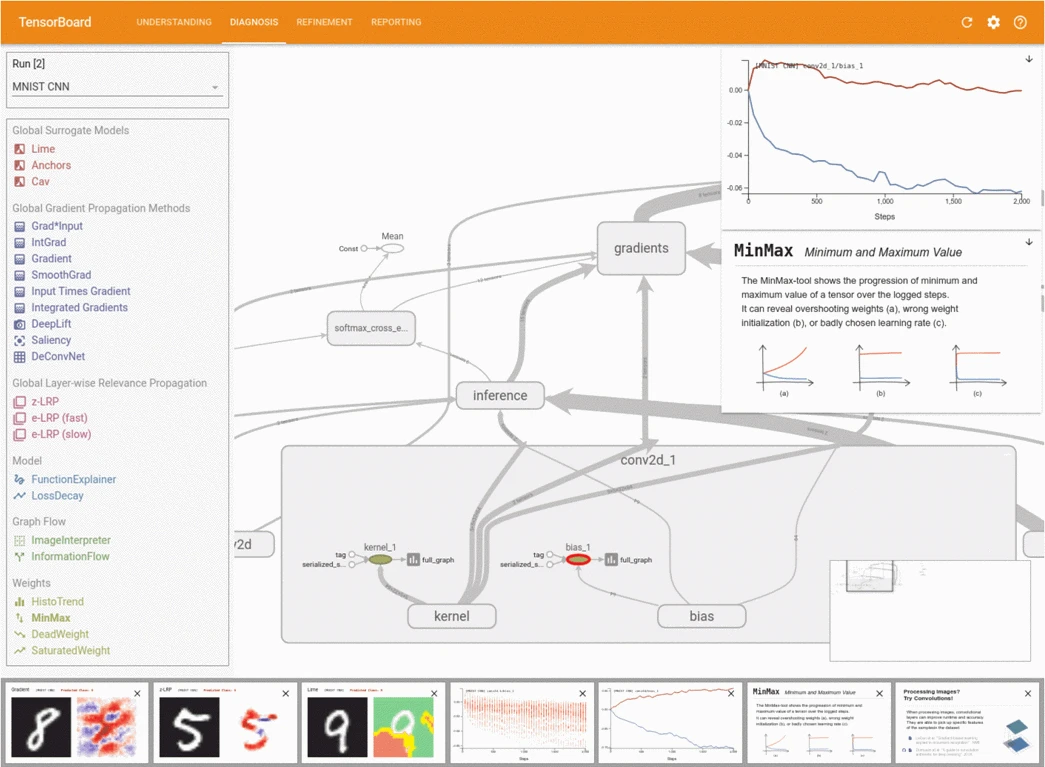
\includegraphics[width=\textwidth]{images/eXplainer dashboard.png}
        \caption{The diagnosis dashboard. Explainers are arranged in a
toolbox-like interface, ordered descending, from high-abstraction to
low-abstraction. The graph visualization provides an overview of the
full model and allows for node selection. Explanations are shown in
the upper toolcard, while information about the explainer is displayed
beneath. The provenance bar contains cards from interesting findings}
        \label{fig:eXplainer_dashboard}
    \end{subfigure}
    \hfill
    \begin{subfigure}[c]{0.39\textwidth}
        \centering
        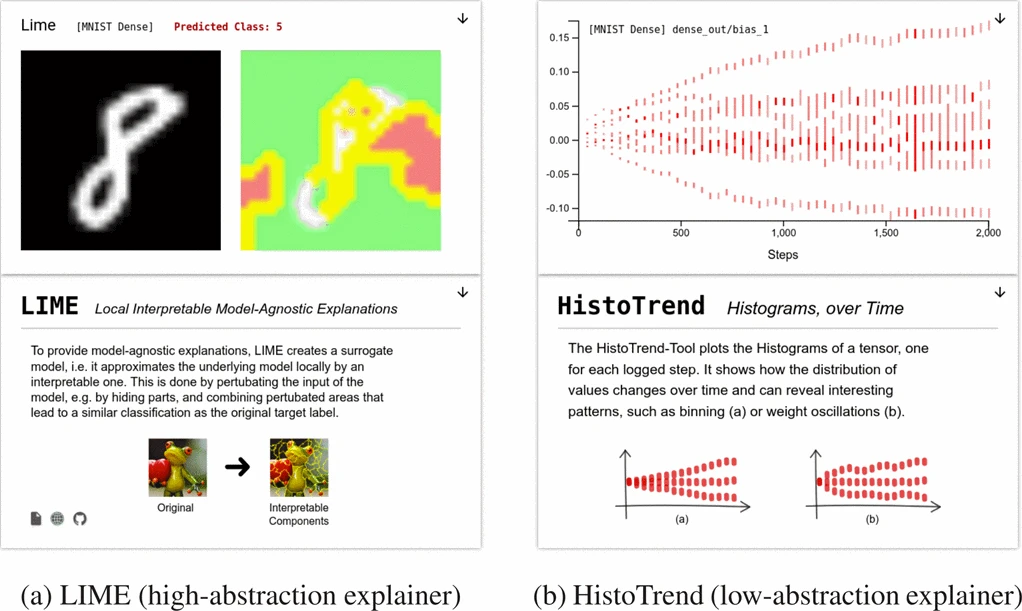
\includegraphics[width=\textwidth]{images/eXplainer card.png}
        \caption{Information cards showing results for different explainers (top)
with the corresponding descriptions for the explainer itself (bottom).}
        \label{fig:eXplainer_cards}
    \end{subfigure}
    \caption{eXplainer interface.}
    \label{fig:eXplainer}
\end{figure}

The framework incorporates eight global monitoring and steering mechanisms that support the overall explanation process, including model quality monitoring, search space exploration, data shift scoring, comparative analytics, provenance tracking, XAI Strategies, knowledge generation, and reporting capabilities. These mechanisms provide essential infrastructure for maintaining context and continuity across extended explanation sessions, allowing users to track their investigation process and build cumulative understanding over time.

From a visualization perspective, explAIner employs a toolbox-based interface, shown in Figure \ref{fig:eXplainer_dashboard}, where explainers are arranged by abstraction level, allowing users to progressively examine the results from high-level model understanding to detailed component analysis. The system's integration with TensorBoard's graph visualization provides a familiar foundation for users already working with deep learning models, while overlay cards, represented in Figure \ref{fig:eXplainer_cards}, present explanatory results and supplementary information based on context.

\paragraph{XAutoML: Transparency for Automated Machine Learning}

While explAIner focuses on manually developed deep learning models, \textbf{XAutoML} \cite{Z_ller_2023} addresses the understanding and of automated machine learning (AutoML) systems. 

% Source: XAutoML paper, page 15
\begin{figure}[ht!]
\centering
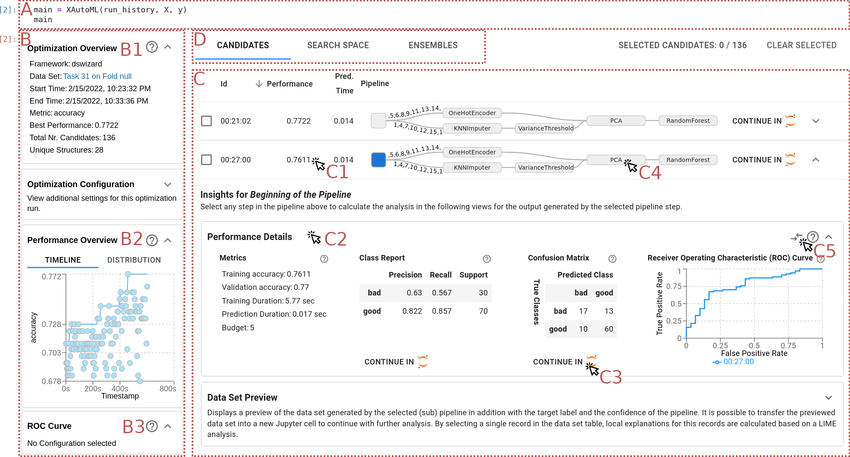
\includegraphics[width=\textwidth]{images/Overview-of-XAutoML-A-The-visualization-is-integrated-with-Jupyter-and-can-be-accessed.png}
\caption{Overview of XAutoML. The visualization is integrated with Jupyter and can be accessed with a few lines of code (A). On the
left side (B), the optimization overview provides basic statistics about the optimization run (B1), a scatter plot of the accuracy of all
candidates over time (B2), and a receiver operating characteristic (ROC) curve of selected candidates (B3, hidden). The leaderboard
view (C, partially hidden) provides a comprehensive overview of all evaluated candidates. Users can open single candidates (C1) in
an overlay on the right-hand side to reveal detailed information about them (only partially visible). The candidate details contain
various boxes grouping related information together. In the performance details view (C2), performance metrics and basic performance
visualizations are available. By clicking the Continue in Jupyter button (C3), the according information can be exported to a new
Jupyter cell. Users can access the search space and ensemble inspection via the tabs at the top (D).}

\label{fig:xautoml_overview}
\end{figure}

The widespread use of AutoML tools produced high-performing models that do not reveal the processes or design decisions behind the obtained pipelines.
XAutoML tackles this challenge through a comprehensive visual analytics approach embedded within JupyterLab, providing four primary views that cover different aspects of the AutoML process. As shown in Figure \ref{fig:xautoml_overview}, the \textit{optimization overview} provides high-level insights into the AutoML run, including performance trajectories over time, candidate distribution by performance, and ROC curve comparisons for selected models. The \textit{candidate inspection} view enables detailed analysis of individual ML pipelines, through XAI techniques such as surrogate models, feature importance analysis, and partial dependence plots.

% Source: XAutoML paper, page 16
\begin{figure*}[htbp]
    \centering
    
    \begin{subfigure}[t]{0.48\textwidth}
        \centering
        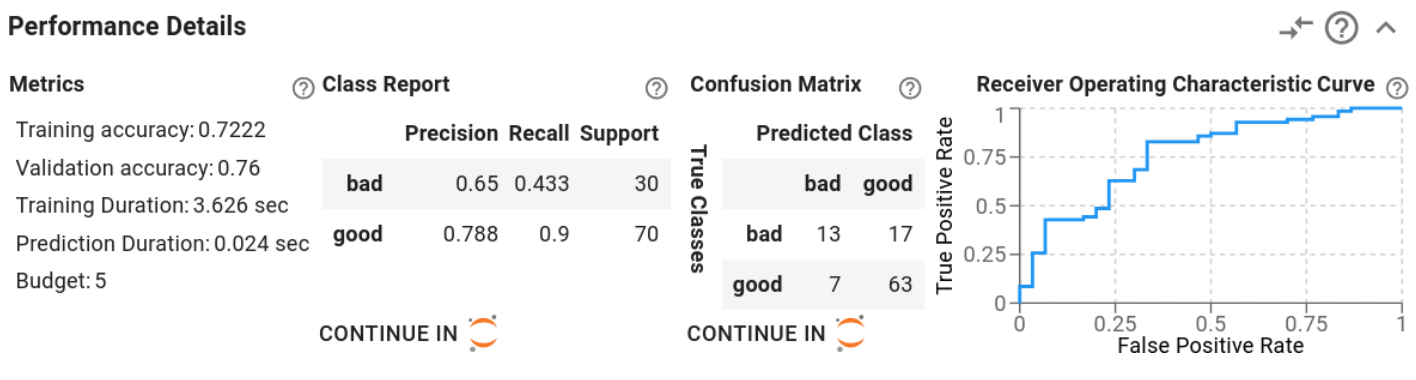
\includegraphics[width=\textwidth]{images/XAutoML a.png}
        \caption{Performance details. From left to right some basic metrics, a class report, a confusion matrix and a ROC curve is displayed.}
        \label{fig:performance_details}
    \end{subfigure}
    \hfill
    \begin{subfigure}[t]{0.48\textwidth}
        \centering
        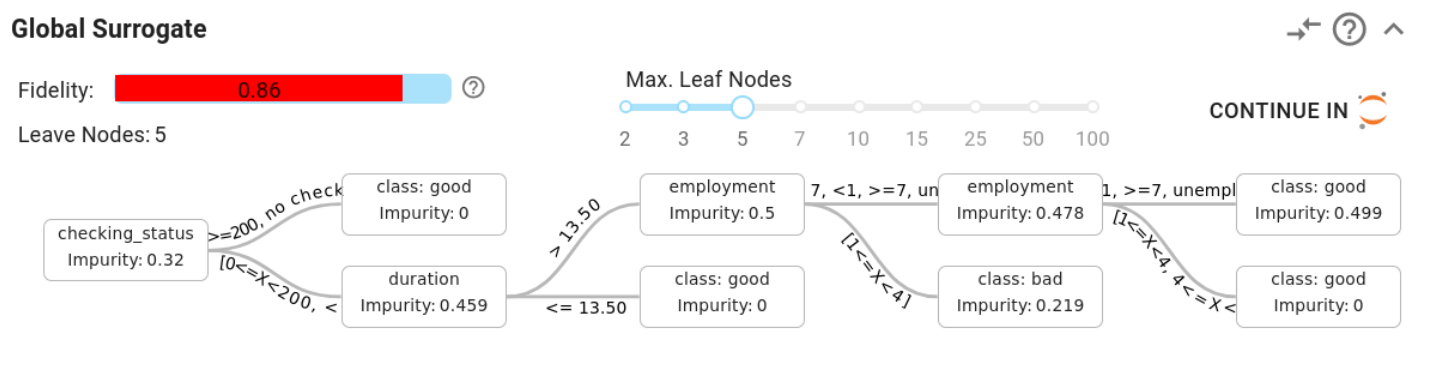
\includegraphics[width=\textwidth]{images/XAutoML b.png}
        \caption{Global surrogate. A decision tree is rendered as a global surrogate. Using the top slider, the tree complexity can be controlled.}
        \label{fig:global_surrogate}
    \end{subfigure}
    
    \vspace{0.5cm}
    
    \begin{subfigure}[t]{0.48\textwidth}
        \centering
        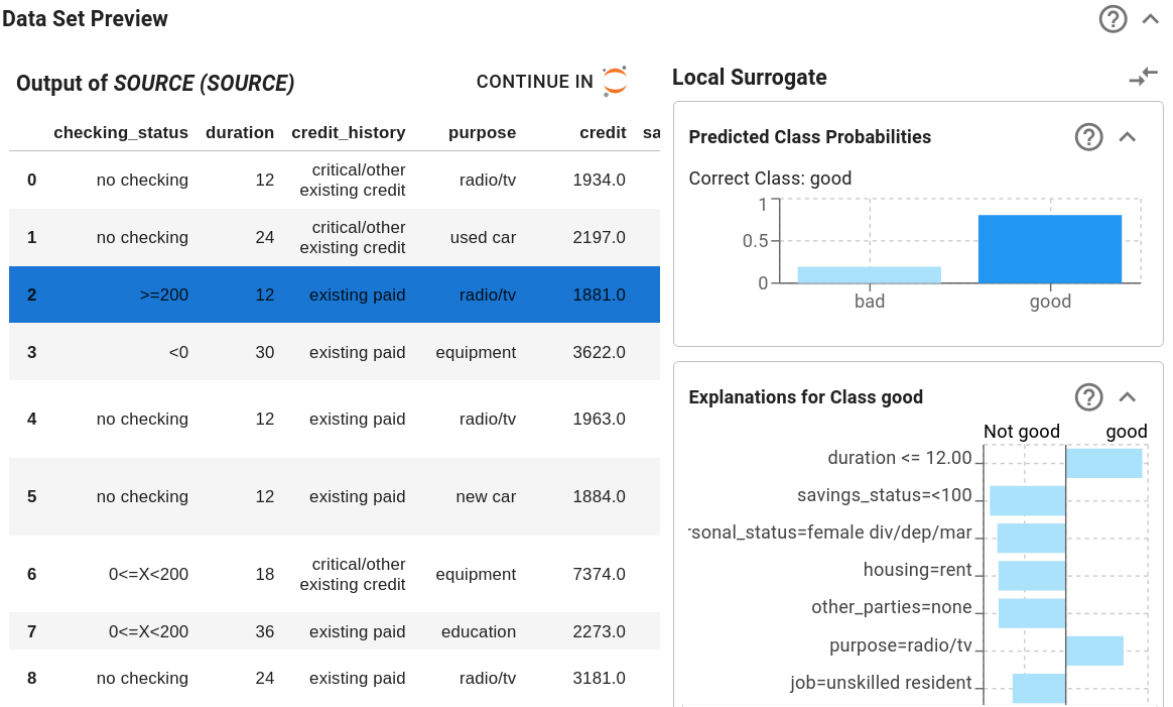
\includegraphics[width=\textwidth]{images/XAutoML c.png}
        \caption{Dataset preview and local surrogate. The left-hand side displays a preview of the input dataset. On the right-hand side feature attributions for the selected sample are displayed.}
        \label{fig:dataset_preview}
    \end{subfigure}
    \hfill
    \begin{subfigure}[t]{0.48\textwidth}
        \centering
        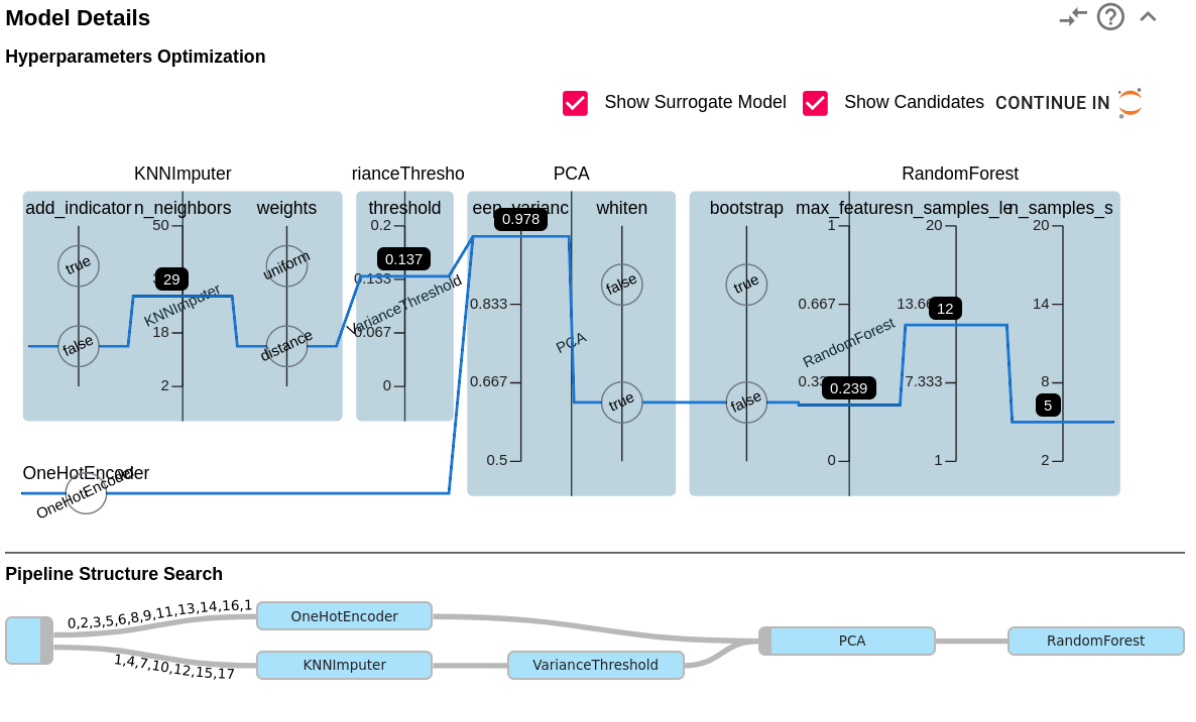
\includegraphics[width=\textwidth]{images/XAutoML d.png}
        \caption{Model details. At the top, the selected hyperparameter configuration is displayed in a CPC. At the bottom, the aggregated structure search graph up to this candidate is rendered.}
        \label{fig:model_details}
    \end{subfigure}
    
    \vspace{0.5cm}
    
    \begin{subfigure}[t]{0.48\textwidth}
        \centering
        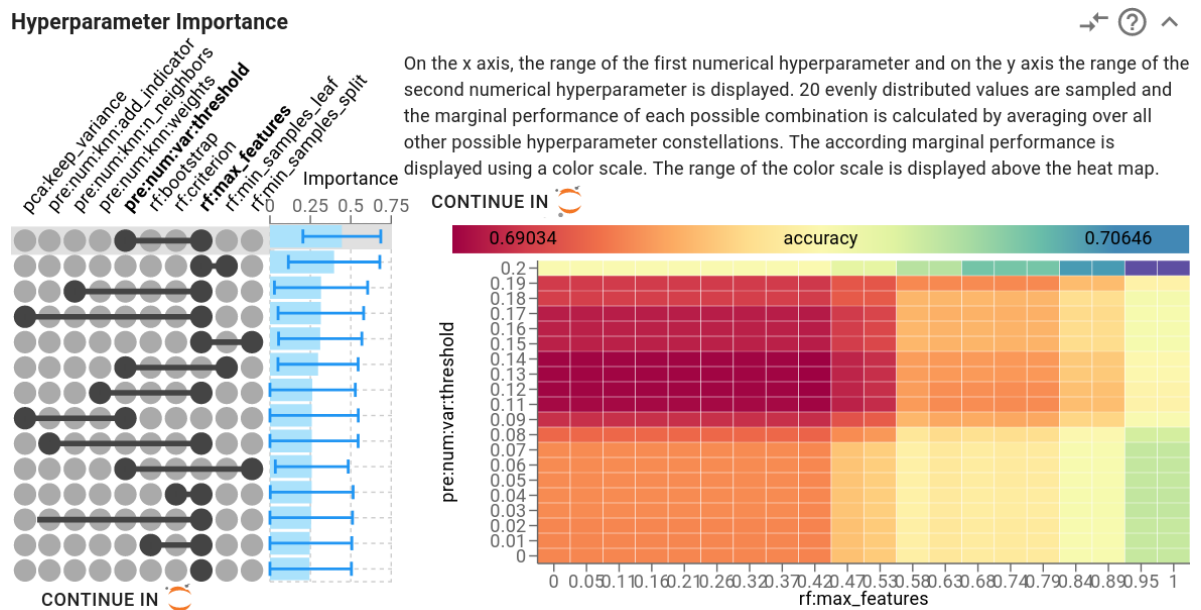
\includegraphics[width=\textwidth]{images/XAutoML e.png}
        \caption{Hyperparameter importance with well-performing regions. On the left-hand side hyperparameter (pairs) are ranked by their importance. On the right-hand side a heat map with well-performing regions of the currently selected hyperparameter pair is displayed.}
        \label{fig:hyperparameter_importance}
    \end{subfigure}
    \hfill
    \begin{subfigure}[t]{0.48\textwidth}
        \centering
        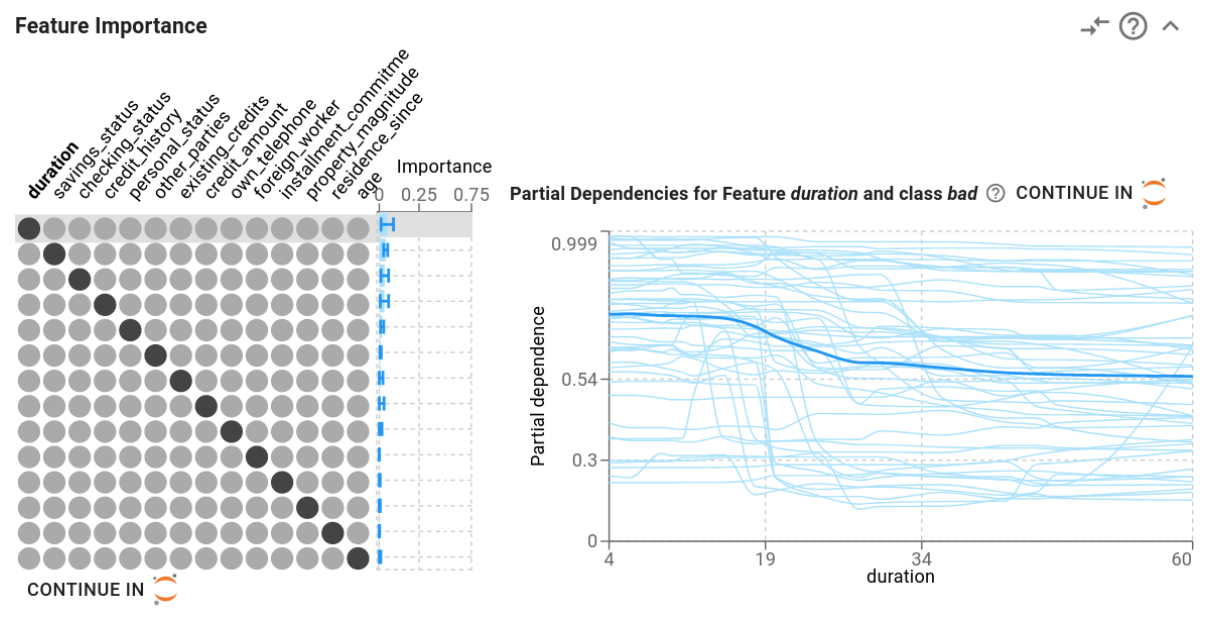
\includegraphics[width=\textwidth]{images/XAutoML f.png}
        \caption{Feature importance with PDP and ICE. On the left-hand side the features are ranked by their importance. On the right-hand side a PDP and ICE plot show the correlation between the feature value and predicted class for the currently selected feature.}
        \label{fig:feature_importance}
    \end{subfigure}
    
    \caption{Overview of visualizations used to explain and validate a single candidate.}
    \label{fig:xautoml_detailed_views}
\end{figure*}

Figure \ref{fig:xautoml_detailed_views} demonstrates the comprehensive nature of XAutoML's explanation capabilities, showing how the system integrates multiple established XAI techniques within a unified interface. The performance details view (a) provides standard validation metrics alongside confusion matrices and ROC curves. The global surrogate view (b) employs decision trees as interpretable approximations of complex models, with user-controllable complexity through a slider interface. The dataset preview and local surrogate view (c) combines data inspection with SHAP-based feature attributions for selected instances.
XAutoML is designed to work smoothly with existing data science workflows by embedding into JupyterLab and offering flexible export options, so users can easily move models, datasets, and analysis results back into their coding environments. The system employs a hierarchical information presentation strategy that helps users avoid cognitive overload while revealing technical details step by step. Domain experts can configure simplified views that hide complex ML details, while comprehensive technical information, including hyperparameter configurations, pipeline structure visualizations, and detailed performance metrics, is available to more experienced users.

% \paragraph{Comparative Analysis and Design Implications}

% Both explAIner and XAutoML demonstrate the feasibility and value of comprehensive XAI frameworks, though they address different segments of the machine learning ecosystem.

% Several design patterns emerge from these frameworks that are relevant to a possible $\text{LORE}_{sa}$ visualization design. First, both systems employ modular architectures that allow diverse explanation methods to be integrated. Second, they emphasize workflow integration rather than standalone analysis, recognizing that explanation is most effective when embedded within existing development and analysis processes. Third, they provide multiple abstraction levels and progressive disclosure mechanisms to accommodate users with varying expertise levels.


\subsubsection{Local Explanation Analysis Tools}

Specialized tools that focus specifically on local explanation analysis have emerged to address the challenge of understanding individual predictions and the underlying decision pattern. 
Two notable examples of specialized local explanation analysis tools are SUBPLEX and FIPER, each addressing different aspects through innovative visual analytics approaches.

\paragraph{SUBPLEX: Subpopulation-Level Local Explanation Analysis}

% \textbf{SUBPLEX} 
\cite{9861728} presents a new approach to understanding local model explanations by analyzing them at the subpopulation level rather than treating individual explanations in isolation. The tool addresses a fundamental limitation in traditional local explanation analysis: while methods like LIME \cite{ribeiro2016should} and SHAP \cite{lundberg2017unified} provide feature importance vectors for individual instances, aggregating these explanations across entire datasets through simple averaging can be misleading, as important patterns may only emerge within specific subgroups of the data.

% Source: SUBPLEX paper, page 6
\begin{figure}
\centering
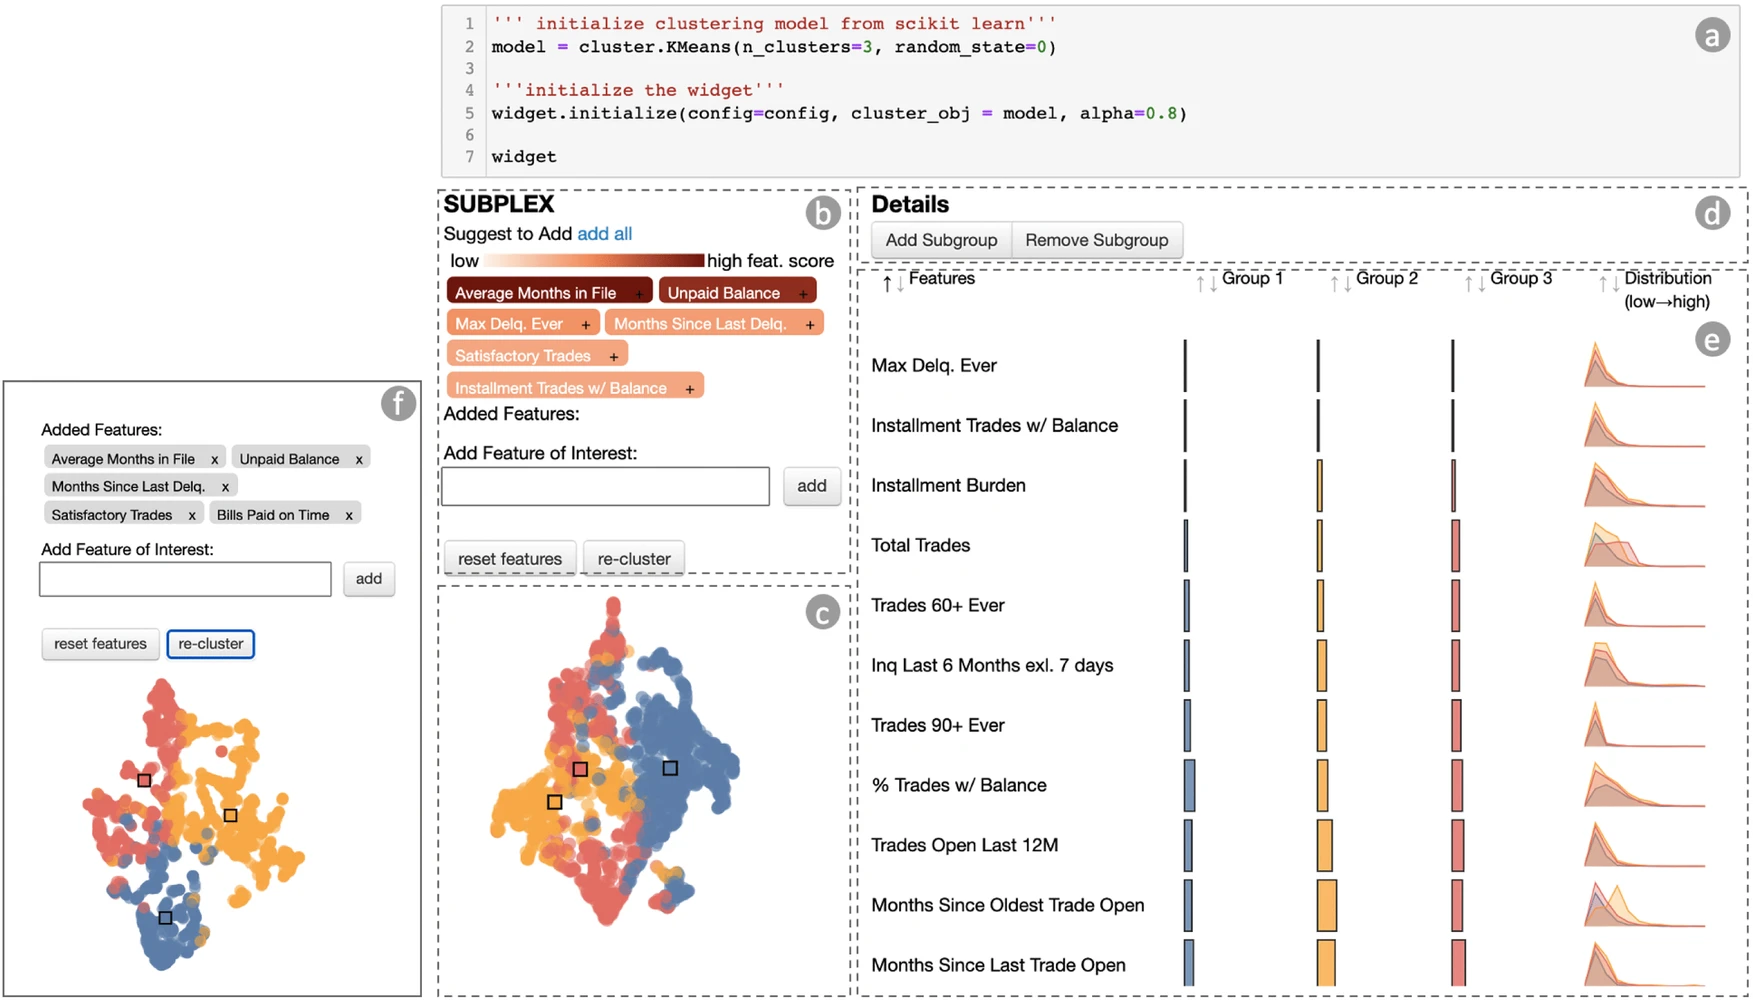
\includegraphics[width=\textwidth]{images/subplex.png}
\caption{SUBPLEX contains five linked views: (a) code block, (b) cluster refinement view, (c) projection view, (d) subpopulation
creation panel, (e) local explanation detail view}
\label{fig:subplex_interface}
\end{figure}

The core innovation of SUBPLEX lies in its human-in-the-loop framework that combines automatic clustering and projection techniques with intelligent user guidance to enable pilotable subpopulation analysis. 
The system addresses the challenge that straightforward application of clustering and projection algorithms to local explanation vectors often fails to reveal meaningful patterns due to the specific characteristics of explanation data, including high dimensionality, sparsity, and varying scales across features.

SUBPLEX implements a three-stage pipeline for subpopulation analysis: \textit{generation}, \textit{exploration}, and \textit{interpretation}. During the generation phase, the system performs automatic clustering of local explanation vectors and provides feature suggestions to guide users toward potentially interesting subpopulations. The clustering process employs K-means for computational efficiency, while UMAP projection is used to visualize the distribution of explanations in a 2D space, enabling users to understand the spatial relationships between different explanation patterns.

% Source: SUBPLEX paper, page 10
\begin{figure}[htbp]
\centering
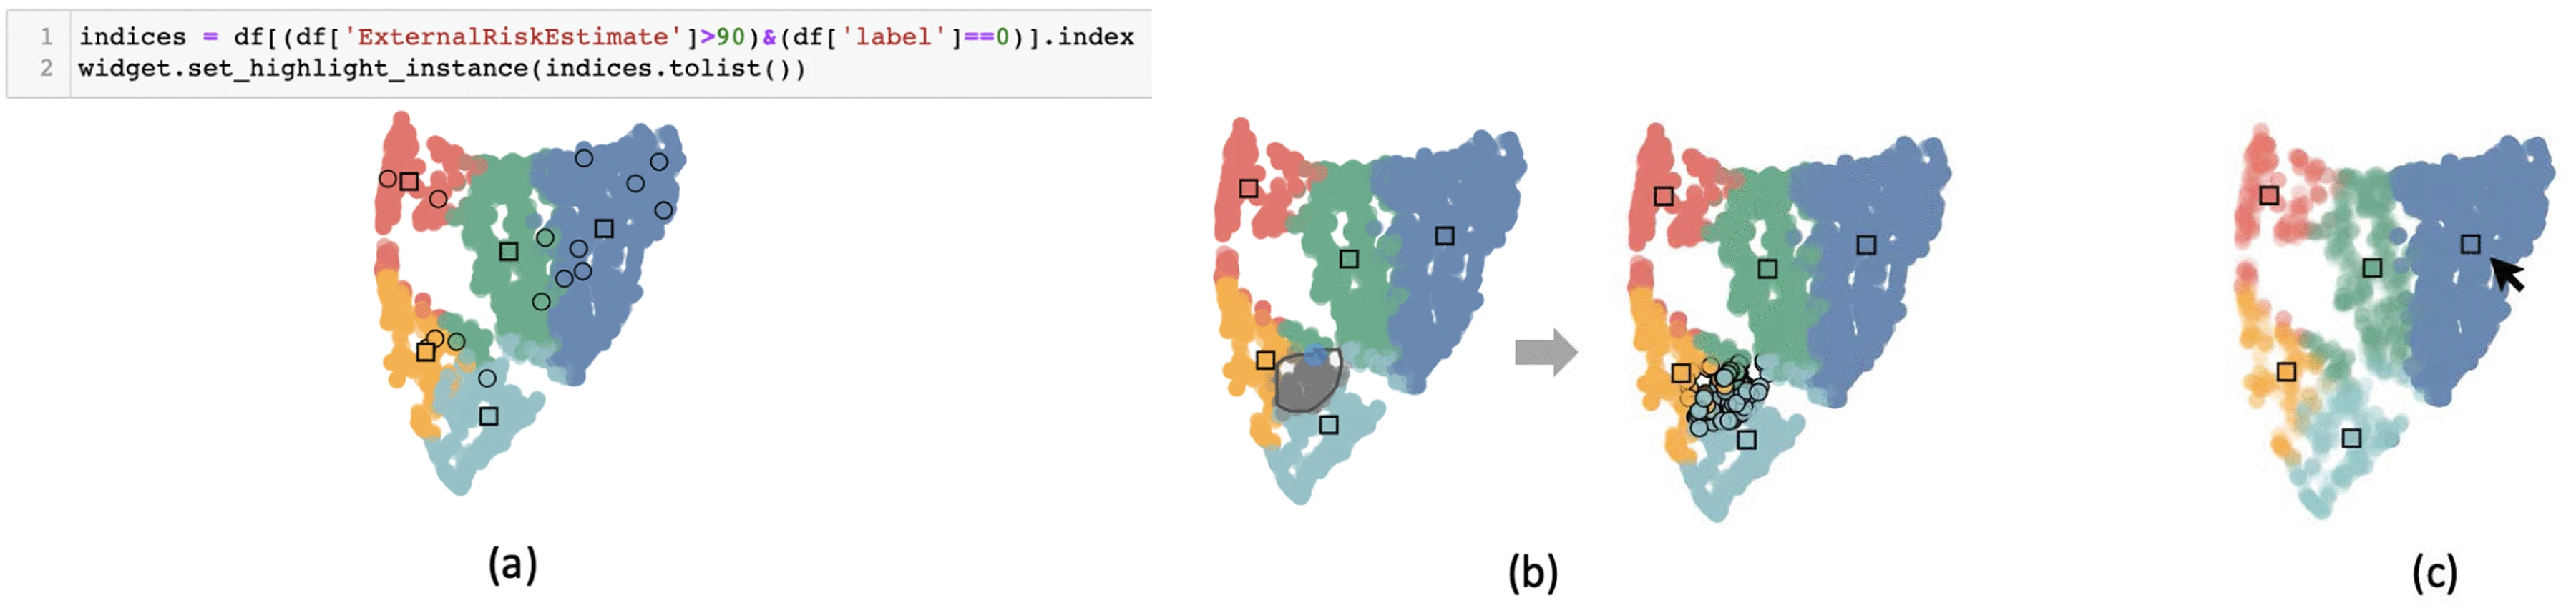
\includegraphics[width=\textwidth]{images/subplex2.png}
\caption{Three methods of selecting/creating a subpopulation for inspection. (a) Highlight instances by coding. (b) Select
instances by brushing. (c) Highlight a cluster by clicking centroid.}
\label{fig:subplex_interactions}
\end{figure}

The exploration phase supports both automatic subpopulation discovery and manual subpopulation creation through multiple interaction mechanisms, as illustrated in Figure \ref{fig:subplex_interactions}. Users can highlight instances by coding, select regions through brushing interactions, or click cluster centroids to define subpopulations of interest. This flexibility acknowledges that domain experts often have specific hypotheses about interesting subgroups that may not be captured by automatic clustering algorithms.

During the interpretation phase, SUBPLEX enables comparative analysis of explanation patterns across subpopulations through bar charts that visualize aggregated local explanations. The system provides export capabilities that allow users to extract intermediate results as variables within Jupyter notebooks, supporting integration with broader data science workflows.

From a visualization perspective, SUBPLEX employs a five-view coordinated interface embedded within Jupyter notebooks, as shown in Figure \ref{fig:subplex_interface}. The projection view shows the distribution of local explanations in 2D space using UMAP, with color encoding to distinguish different subpopulations. The cluster refinement view provides feature suggestions and enables iterative cluster refinement through feature selection. The subpopulation creation panel supports manual manipulation of subgroups, while the local explanation detail view presents aggregated explanation patterns for selected subpopulations.

\paragraph{FIPER: Hybrid Rule and Feature Importance Visualization}

% \textbf{FIPER} 
\cite{cappuccio2024fipervisualbasedexplanationcombining} addresses a different challenge in the analysis of local explanations by combining rule-based explanations with feature importance methods within a merged visual interface. The tool recognizes that rule-based explanations provide comprehensive logical predicates that fully describe the conditions leading to specific predictions, but it can be cognitively demanding to process. Conversely, feature importance methods like SHAP \cite{lundberg2017unified} provide lightweight, easily interpretable rankings even though they offer less detailed information about decision boundaries.

% Source: FIPER paper, page 5
\begin{figure}[ht!]
\centering
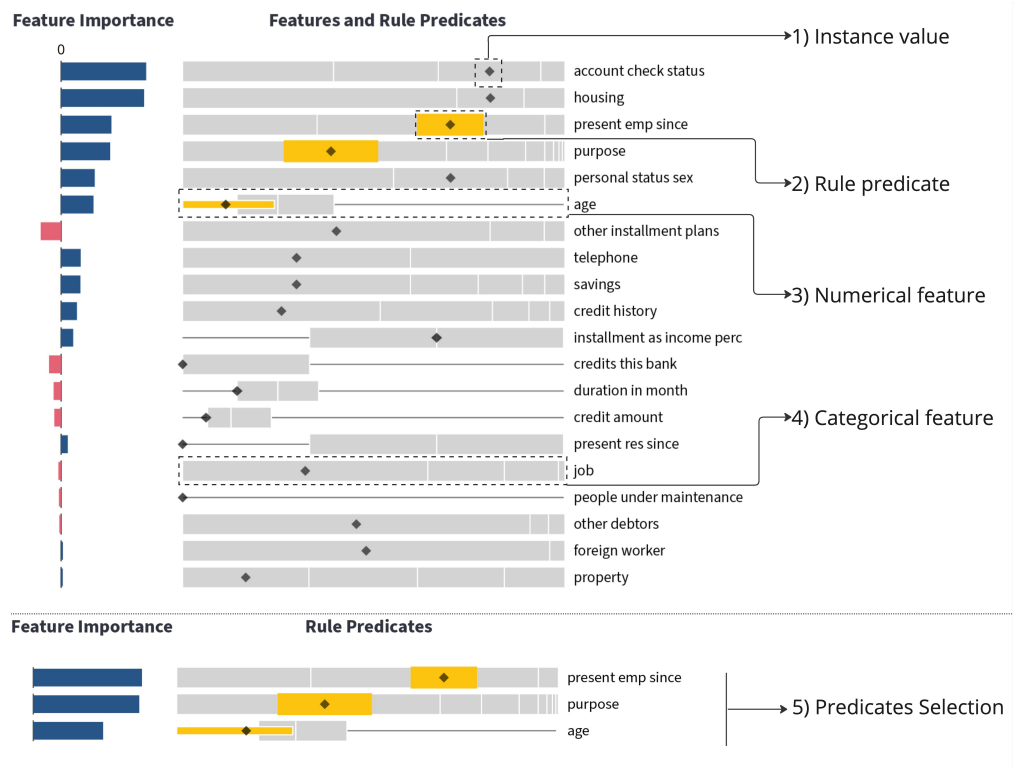
\includegraphics[width=\textwidth]{images/FIPER 1.png}
\caption{FIPER visualization of one instance of the German Credit Risk dataset. Top panel: Attributes are sorted by the absolute value of feature importance (FI). Categorical attributes are represented as stacked bar charts. Numerical values are represented as box plots with quartile information. The intervals contained in the predicates of the rule are highlighted in yellow. Bottom panel: Filtered view of the visualization, showing only the attributes referred to in the rule premise, demonstrating the system's ability to focus user attention on rule-relevant features.}
\label{fig:fiper_interface}
\end{figure}

FIPER's central contribution is its hybrid approach that uses feature importance rankings to organize and prioritize the presentation of the rule-based explanation. The system employs LORE \cite{guidotti2022stable, guidotti2019lore} for rule generation and SHAP \cite{lundberg2017unified} for feature importance calculation, though the architecture is designed to accommodate other rule-generating algorithms (such as Anchors \cite{10.5555/3504035.3504222}) and alternative feature importance methods (such as LIME \cite{ribeiro2016should}).

As shown in Figure \ref{fig:fiper_interface}, the visualization organizes the explanation space into two coordinated panels. The left panel presents feature importance weights sorted by their absolute values, using color coding to indicate positive (blue) or negative (magenta) contributions to the prediction. The right panel visualizes rule predicates in an order that follows the feature importance ranking, ensuring that the most relevant features are presented first to users.

% Source: FIPER paper, page 6
\begin{figure}[ht!]
\centering
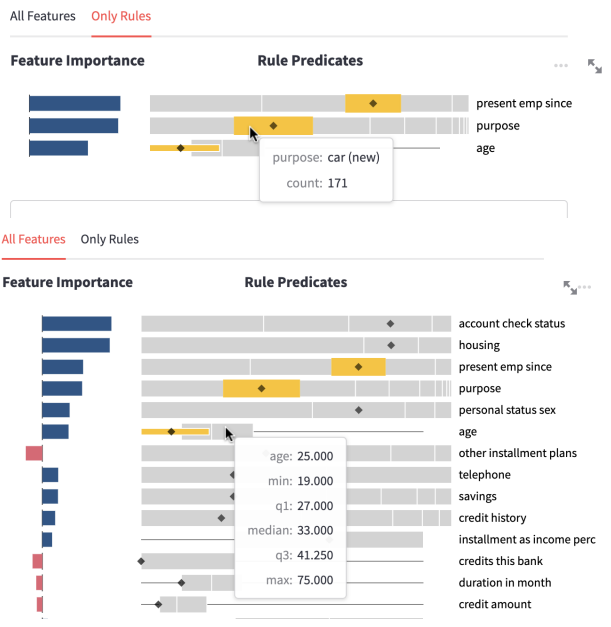
\includegraphics[width=0.9\textwidth]{images/FIPER 2.png}
\caption{Detailed feature information accessible by hovering over specific features: Top panel shows tooltip for a categorical data type, displaying the feature's actual value with its class cardinality information. Bottom panel shows a tooltip for a numerical data type, presenting statistical central values including minimum, maximum, median, first quartile (Q1), and third quartile (Q3).}
\label{fig:fiper_details}
\end{figure}

FIPER employs differentiated visualization strategies based on feature types to maximize information density while maintaining clarity. For categorical features, the system uses stacked bar charts to show the part-of-the-whole relationship of possible values, with diamond markers indicating the observed value for the current instance. For numerical features, box plots provide a compact visualization of data distributions, including quartiles, median, and range information, with highlighted intervals showing the rule predicate ranges.

The system incorporates two forms of interactivity to support the exploration, as illustrated in Figure \ref{fig:fiper_details}. Users can dynamically restrict the view to show only features mentioned in rule predicates, following the principle of providing easy access to relevant information. Additionally, hovering interactions reveal detailed distribution information for specific features, including cardinality for categorical variables and statistical summaries for numerical variables.

A controlled user study comparing FIPER with textual LORE output and an enhanced XAI library visualization demonstrated 
that while FIPER required slightly more time for task completion, it substantially improved accuracy across all tasks, even with complex instances. User feedback indicated that FIPER was considered more understandable and valuable, with 10 out of 15 participants selecting it as their preferred visualization approach.

The study also revealed new insights into user preferences. While FIPER demonstrated superior performance for datasets with many features, some participants suggested that simpler visualizations might be more appropriate for datasets with fewer attributes. This finding highlights the importance of adaptive visualization strategies that can scale appropriately with data complexity.

\subsubsection{Surrogate Model Visualization Tools}

Surrogate model visualization represents a distinct category within vXAI, focusing specifically on the interpretable models that approximate the behavior of a black box machine learning system. Unlike local explanation analysis tools that examine individual predictions or comprehensive frameworks that integrate multiple explanation modalities, surrogate model visualization tools focus on creating and visualizing simplified models that capture the essential decision-making patterns.

\paragraph{DeforestVis: Decision Stump-Based Surrogate Analysis}

% \textbf{DeforestVis} 
\cite{Chatzimparmpas2023DeforestVisBA} presents an innovative approach to the visualization of the surrogate model employing decision stumps, decision trees of one level, generated through the AdaBoost \cite{FREUND1997119} algorithm. This approach addresses a critical limitation in traditional surrogate model approaches: while full decision trees can become prohibitively complex when attempting to approximate sophisticated target models, and rule sets can become unwieldy with numerous if-else statements, decision stumps provide a middle ground that maintains interpretability while capturing essential decision patterns.

The system's core lies in its recognition that ensemble methods like AdaBoost naturally decompose complex decision boundaries into collections of simple, weighted decision stumps. Rather than attempting to visualize a single complex surrogate model, DeforestVis takes advantage of this decomposition to provide multiple levels of abstraction: users can examine individual stumps for detailed understanding, analyze feature-based aggregations for intermediate insights, or observe overall model behavior for high-level comprehension.

% Source: DeforestVis paper, page 3
\begin{figure}[ht!]
\centering
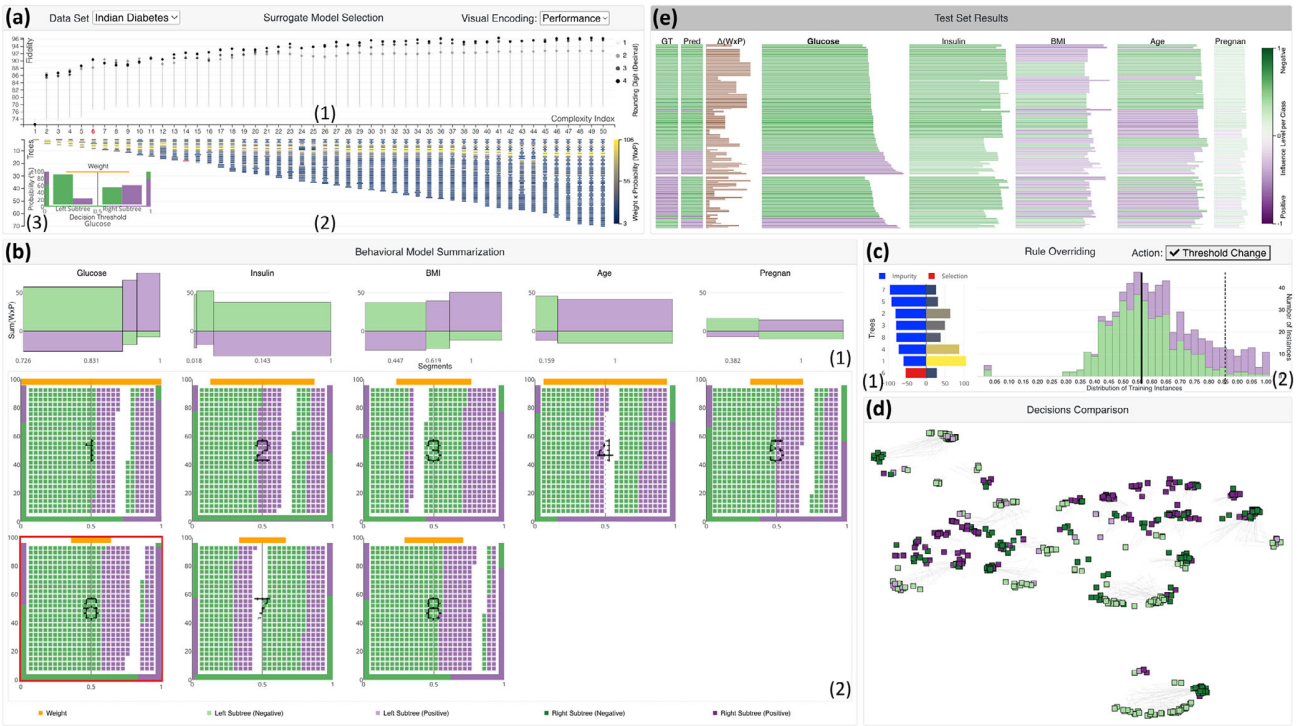
\includegraphics[width=\textwidth]{images/DeforestVis.png}
\caption{Components of DEFORESTVIS: (a.1) lollipop plot shows data-rounding effects in the fidelity score for four different decimal digit
precisions; (a.2) dot plot with lines of various widths (unique rules/stumps > original > duplicated) and colors (visual encoding: performance,
that is, weighted probability (W × P)) that explains complexity increase as more decision stumps get added and (a.3) selective stump-based
explanation; (b.1) segmented bar chart tells the predictive outcome and power of each segment based on automatically computed thresholds
and (b.2) detailed stump-based explanation grid; (c.1) bar chart shows the impurity and weighted probability of each decision stump; (c.2)
histogram shows the active rule’s threshold and distribution of training instances; (d) projection aggregates the global behaviour of instances;
colour shows the local behaviour according to the currently selected decision stump; and (e) fragmented bar chart shows the per-feature
contribution and influence level for each test case.}
\label{fig:deforestvis_interface}
\end{figure}

DeforestVis implements a five-view coordinated interface that supports a comprehensive workflow for surrogate model analysis, as illustrated in Figure \ref{fig:deforestvis_interface}. The \textit{surrogate model selection} view enables users to explore the complexity-fidelity trade-off by incrementally adding decision stumps to the ensemble while monitoring performance metrics. This view is particularly useful for its visualization of the relationship between model complexity (number of stumps) and surrogate fidelity (accuracy in approximating the target model), allowing users to identify optimal points where additional complexity provides diminishing returns.
The \textit{behavioral model summarization} view aggregates decision stumps by feature, providing users with feature-level insights into the target model's decision patterns. This aggregation approach addresses the cognitive challenge of interpreting large numbers of individual stumps by organizing them according to the features they split on, enabling users to understand which features the target model considers most important and how their decision boundaries are constructed.
The \textit{rule overriding} and \textit{decision comparison} views enable users to manually adjust decision thresholds within individual stumps and immediately observe both local and global impacts of their modifications. The local impact analysis shows how threshold changes affect specific training instances, while global impact analysis demonstrates broader effects on model predictions across the entire dataset. This allows domain experts to fine tune the automatically generated rules, potentially improving both model performance and interpretability.
The \textit{test set results} view provides validation capabilities that allow users to assess the effectiveness of their manual modifications on unseen data. This view supports case-by-case analysis, enabling users to understand why specific instances received particular classifications based on the contribution of each feature as encoded in the ensemble of decision stumps.

From a technical perspective, DeforestVis employs the Explainable Boosting Machine (EBM) as its target model, chosen specifically because it produces systematically fewer decision rules compared to other ensemble methods like XGBoost or Random Forest. However, the system's workflow remains model-agnostic, as AdaBoost-based surrogate models can approximate the behavior of any machine learning model, making the approach broadly applicable across different modeling contexts.
The system's evaluation through expert interviews with data analysts and model developers revealed key insights. Experts particularly appreciated the multi-level transparency that DeforestVis provides, enabling both top-down analysis (starting from overall model behavior) and bottom-up investigation (beginning with individual decision stumps). 
